\ssection{Deslocamento e Transporte}	
    \ssubsection{Ônibus Internos (Circulares)}
    A UFRJ conta com ônibus circulares gratuitos que rodam por todo o campus do Fundão. Há três linhas, sendo duas delas as que servem para você que vai para o bloco H do Centro de Tecnologia.
    
    Há algumas dicas, inclusive de boa convivência, para o uso dos circulares: durante o início do período, a quantidade de alunos que pegam esses ônibus aumenta muito e, por conta disso, estes ficam muito lotados. Em geral, para um melhor proveito do sistema, podemos tomar algumas atitudes que melhoram a nossa viagem de cada dia. Seguem algumas delas:
    \begin{itemize}
    	\item[-] Não fique na porta se o meio do ônibus está vazio
        \item[-] Evite deixar a mochila nas costas, pois ocupa mais espaço e atrapalha as outras pessoas
        \item[-] Se você estiver sentado, ofereça-se para segurar a mochila de alguém que está em pé
    \end{itemize}
    
    Abaixo, você pode ver as rotas de cada uma das linhas de circular. \textbf{Vale ressaltar que os ônibus, a partir de 19h, vão até a estação do BRT}.
    
    Para você, nosso calouro, o ponto mais próximo do nosso bloco não é o ponto do CCMN/CT Bloco A, como muitos pensam. Nosso bloco, sendo o último do CT, fica no ponto seguinte (Letras/CT Bloco H). Porém, fique atento, pois as aulas de Física Experimental são no Bloco A, então, nesse caso, é melhor saltar no ponto CCMN/CT Bloco A.
    
    Para maiores informações sobre as linhas, pontos de ônibus e afins, você pode consultar o site da Prefeitura Universitária: \href{http://www.prefeitura.ufrj.br/index.php/pt/transporte-integrado}{http://www.prefeitura.ufrj.br/index.php/pt/transporte-integrado}

       
    	\ssubsubsection {Circular 1 (Estação UFRJ x Gráfica UFRJ)}
        
        Diário, das 5h à meia-noite.
        
        \begin{center}
          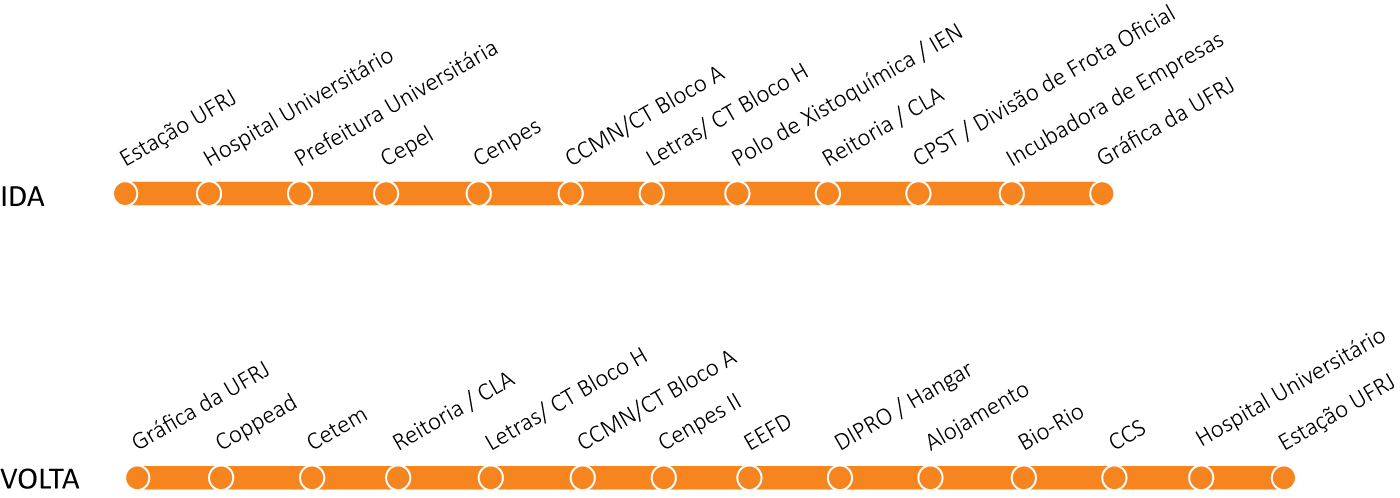
\includegraphics[width=\textwidth]{assets/esquematico_circular1_ufrj.png}
    	\end{center}               
		      
         \pagebreak
              
         \ssubsubsection {Circular 2 (Estação UFRJ x COPPEAD)}
        
        Segunda a sexta, das 6h às 19h.
        
        \begin{center}
          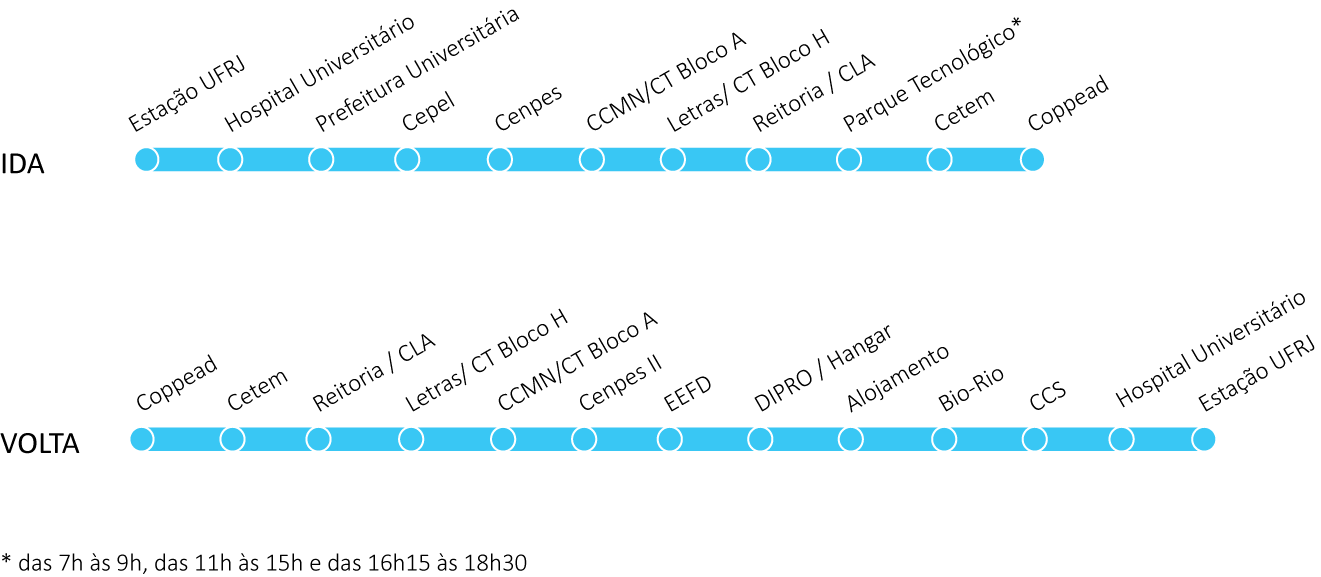
\includegraphics[width=\textwidth]{assets/esquematico_circular2_ufrj.png}
    	\end{center}       
        
        
         \ssubsubsection {Circular 3 (Estação UFRJ x Alojamento)}
        
        Diário, das 5h à meia-noite.
        
        \begin{center}
          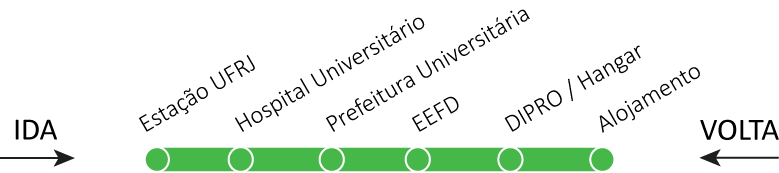
\includegraphics[width=0.6\textwidth]{assets/esquematico_circular3_ufrj.png}
    	\end{center}                               

	
    \ssubsection{Ônibus Intercampi}
    Esses são os ônibus da UFRJ, também gratuitos, que circulam pelos diferentes campi da UFRJ. \textbf{Aqui iremos mostrar nos esquemáticos as paradas fora do Fundão}. Porém, há paradas dentro do Fundão, sendo essas as mesmas dos ônibus circulares. Ou seja, para você, nosso calouro, esses ônibus também param no ponto de Letras/CT Bloco H. Fique atento aos horários, porque costumam ser pontuais.
    \ssubsubsection{Cidade Universitária x Praia Vermelha (Parador)}
        \begin{itemize}
          \item [] Ida: 6h30, 12h15 e 17h15
          \item [] Volta: 12h15, 15h30, 19h e 22h30        
    	\end{itemize}
    
    \begin{center}
          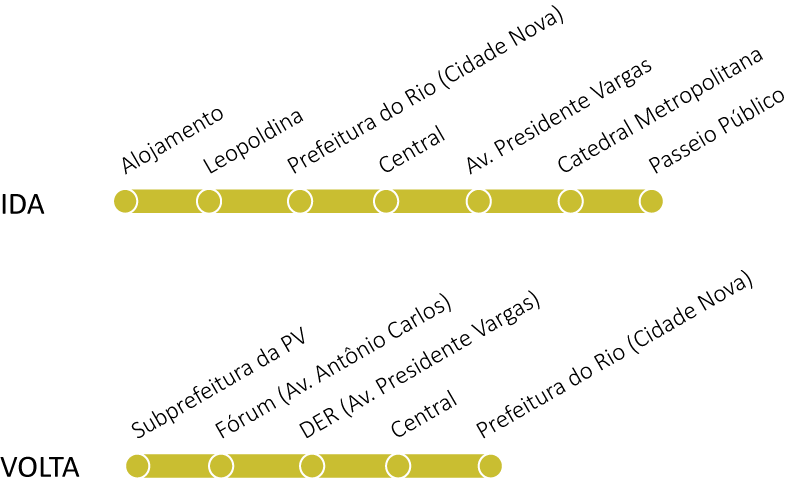
\includegraphics[width=0.7\textwidth]{assets/esquematico_intercampi_pv_ufrj.png}
    \end{center} 
        
    \ssubsubsection{Cidade Universitária x Praia Vermelha (Expresso)}
	\begin{itemize}
            \item [] Ida: 6h30, 12h e 17h15
            \item [] Volta: 13h    
      \end{itemize}
      Essa linha, como diz o nome, tem apenas uma parada, tanto na ida quanto na volta. Tendo como destino a Praia Vermelha, o ponto de partida é o Alojamento no Fundão, parando apenas no Fluminense Futebol Clube e seguindo para o campus da PV (Praia Vermelha). Já quando o destino é a Cidade Universitária, o ônibus parte da Subprefeitura da Praia Vermelha, parando na Prefeitura do Rio (Cidade Nova) e seguindo até o Fundão.

    \ssubsubsection{Cidade Universitária x Praça XV}
      \begin{itemize}
            \item [] Ida: 19h30, 20h30, 21h30 e 22h20
            \item [] Volta: 17h20    
      \end{itemize}
      Vale ressaltar que o horário de 22h20 estende o seu trajeto até a Praia Vermelha
      
      \begin{center}
          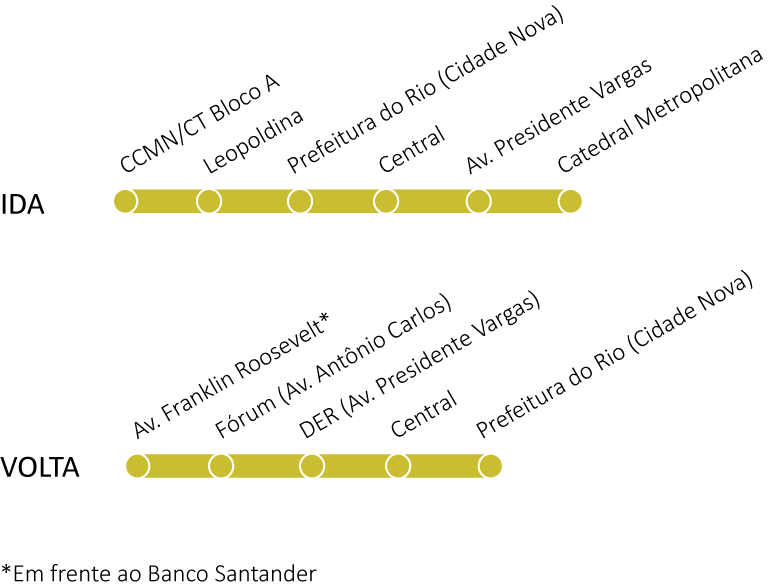
\includegraphics[width=0.7\textwidth]{assets/esquematico_intercampi_pracaXV_ufrj.png}
    \end{center} 
    
    \ssubsubsection{Cidade Universitária x Bonsucesso}
	Esse ônibus circula em apenas três horários: 20h30, 21h40 e 22h20. Porém, fique atento, os horários de 20h30 e 22h20 vão até o Norte Shopping e a estação ferroviária de Cascadura. Infelizmente, não há mais informações sobre a rota no site da Prefeitura Universitária. O ponto de partida é no CCMN/CT Bloco A.
    
    \ssubsection{Ônibus Municipais e Intermunicipais}
    %Levantamento das linhas de ônibus
    \begin{itemize}    	            
        \item Barra da Tijuca
        
        	410 e 420, que são da linha intermunicipal, saindo da Alvorada, direto para o Fundão. Na ida, o ônibus passa no CT, mas na volta é preciso pegá-lo no ponto depois do CCMN, na Linha Amarela
            
        \item Centro/Tijuca
        
        	É possível pegar os ônibus 321, 323, 327 e 485, sendo que os 32x devem ser pegos no ponto Letras/CT Bloco H. Assim, é possível parar na Cidade Nova para pegar outro ônibus para a Tijuca.
            
        \item Ilha do Governador
        
        	Pode-se pegar os ônibus 321, 323, 327, 634, 635, 696 e 910A na ida e parar no BRT. Na volta, é só pegar o ônibus interno até a Estação UFRJ, andar cerca de três minutos até o Terminal do BRT (Aroldo Melodia), pois nesse terminal passam vários ônibus para a Ilha.
            
        \item Zona Norte
        
        616 e 913 - Del Castilho: Vão até o shopping Nova América
        
        945 e 381 - Pavuna: Segue pela Av. Brasil e passam por boa parte da Zona Norte.
        
        \item Zona Oeste
        
        Considerando a grande extensão da Zona Oeste, fizemos um resumo de algumas opções de transporte de lá para o Fundão. É claro que essas não são as únicas opções, mas serve como um guia para você, calouro.
        
        Algumas opções são:
        
        - 410: São João de Meriti
            
        - 420: Nilópolis
            
        - Limousine Carioca: Duque de Caxias
        
        - 936  (Campo Grande x Fundão): Sai da rodoviária de Campo Grande, passa por Santíssimo e segue pela Av. Brasil entrando no Fundão pela Linha Amarela (Em média, são 3h de viagem).
                 
 		- Pegar um trem (Santa Cruz x Central) ou ônibus (790 - Cascadura) até Madureira e lá pegar o BRT em direção ao Fundão (Alvorada x Galeão).
        
 		- Pegar um ônibus (358 - Candelária) ou trem (Santa Cruz x Central) até o Centro e lá embarcar em uma das opções para o Fundão (321, 323, 325, 327).
        
		- Pegar um ônibus até a Av. Brasil e lá embarcar em uma das opções para o Fundão.
        
 		- Pegar o BRT Transoeste até Alvorada (Santa Cruz x Alvorada ou Pingo d’ água x Alvorada) e depois mudar para a linha Alvorada/Fundão (expresso) ou Alvorada/Galeão (semidireto).
        
		- Pegar um trem até a Central (Santa Cruz x Central) e depois pegar o 485 na Cidade Nova.

        \item Zona Sul
        
        Para ir para o Fundão, basta pegar o 485. Em geral, ele cobre toda a Zona Sul, mas, dependendo do bairro que você more, pode ser necessário pegar algum ônibus antes. Por exemplo, no caso de quem mora no fim de Copacabana, quase início de Ipanema, vale a pena pegar qualquer ônibus que passe na Siqueira Campos, para pegar o 485 (é de onde o ônibus sai)
        
        Para sair do Fundão, basta pegar um ônibus que passe pela Cidade Nova (os mais comuns no ponto do H são: 321, 323, 325 e 327). Saltando na Cidade Nova, é possível pegar o 485 no ponto na rua rente aos trilhos do metrô. Geralmente eles passam de 10 em 10 minutos.

        
    \end{itemize}
    
    \ssubsection{BRT}
        O BRT, na teoria, é uma das formas mais fáceis e rápidas de se chegar ao Fundão. São oferecidas três linhas ao Fundão: Expresso Fundão, Semidireto Galeão e Parador Fundão.
        
        A partir do início de 2018, a linha expressa para o Fundão teve seu funcionamento atualizado, existindo apenas em horários específicos, que são: de 4h20 às 9h20 e de 15h25 às 19h10. Fora desses horários, é possível usar o semi-direto Galeão ou o Parador Fundão. Vale ressaltar que, com exceção do parador, as linhas não param em todas as estações da Transcarioca. Abaixo você pode ver os esquemáticos com as estações de parada de cada um dos serviços do BRT Transcarioca.
        \begin{center}
        	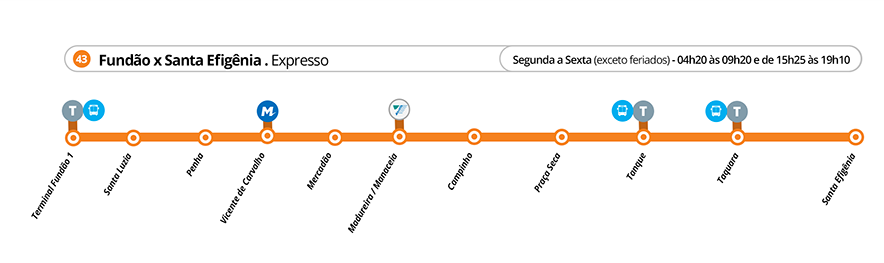
\includegraphics[width=\textwidth]{assets/mapa__transcarioca_expresso.png}
            \captionof{figure}{Estações de parada do serviço Expresso}
        \end{center}
        \begin{center}
        	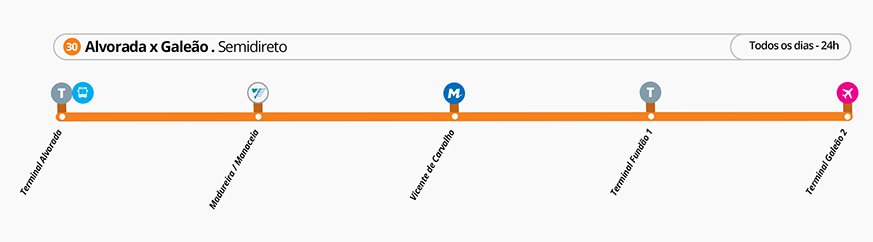
\includegraphics[width=\textwidth]{assets/mapa_transcarioca_semidireto.png}
            \captionof{figure}{Estações de parada do serviço Semidireto}
        \end{center}    
        \begin{center}
        	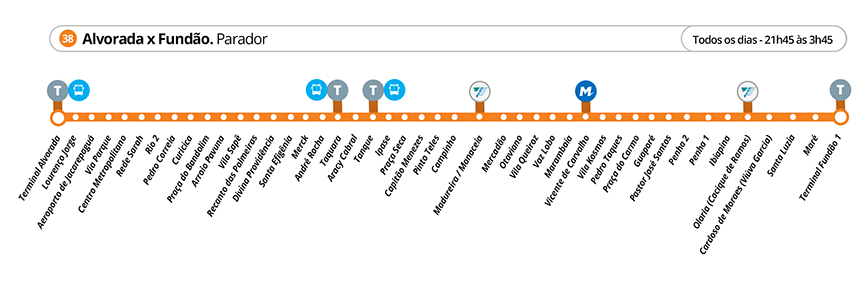
\includegraphics[width=\textwidth]{assets/mapa_transcarioca_parador2.png}
            \captionof{figure}{Estações de parada do serviço Parador Alvorada - Fundão}
        \end{center}
        \begin{center}
        	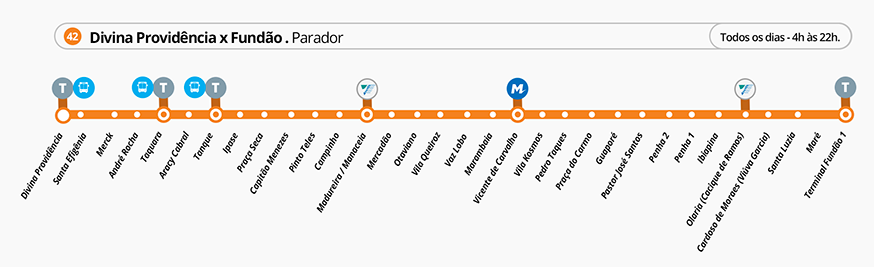
\includegraphics[width=\textwidth]{assets/mapa_transcarioca_parador1.png}
            \captionof{figure}{Estações de parada do serviço Parador Divina Providência - Fundão}
        \end{center}
        
        \ssubsubsection{Algumas dicas sobre o BRT}
            Durante os horários em que não há o serviço expresso, os intervalos entre um ônibus e outro ficam muito grandes, chegando a 25 minutos de espera. Além disso, as estações do serviço expresso ficam muito cheias entre 6h30 e 7h30. Assim, muitas vezes, você acabará não conseguindo entrar no primeiro ônibus que vier. Dessa forma, se você depende desse serviço e tem aulas práticas de manhã com tolerância de atraso (como Física Experimental), programe-se bem ou procure uma carona.
    
    \subsection{Caronas}
    Considerando muitas vezes a dificuldade de locomoção através do transporte público, há uma quantidade grande de alunos que oferecem carona. Em geral, há grupos de caronas específicos para cada bairro. Como forma de auxílio, é cobrado um valor pela carona, que varia de acordo com o grupo. Reunimos aqui algumas informações de grupos de carona que conhecemos.
    
    \begin{itemize}
        \item Barra
            
            Esse é um grupo que vive lotado e, portanto, há um formulário para entrar na lista de espera para poder participar: \href{https://goo.gl/forms/co0jbLLu2KJvuk0D2}{https://goo.gl/forms/co0jbLLu2KJvuk0D2}
            
        \item Vila da Penha/ Vista Alegre/ Olaria
        
            Existe um grupo no \textit{WhatsApp}, mas que depende de algum conhecido para poder te adicionar. É cobrado o valor de R\$4,00 pela carona, por conta de combustível. Não há um \textit{link} público.
        
        \item Niterói
        
            Existe um grupo geral no \textit{Facebook}, \href{https://www.facebook.com/groups/134126660012592/}{Carona Niterói-Fundão}, mas há também grupos no \textit{WhatsApp} que dependem de um conhecido para ser adicionado.
        
        \item Tijuca
        
            Esse grupo também inclui caronas para Grajaú, Vila e Maracanã. A entrada é feita através do seguinte formulário: \href{https://goo.gl/DKJ2nB}{https://goo.gl/DKJ2nB}
        
    \end{itemize}
    
    
    
